% Options for packages loaded elsewhere
\PassOptionsToPackage{unicode}{hyperref}
\PassOptionsToPackage{hyphens}{url}
%
\documentclass[
  ignorenonframetext,
]{beamer}
\usepackage{pgfpages}
\setbeamertemplate{caption}[numbered]
\setbeamertemplate{caption label separator}{: }
\setbeamercolor{caption name}{fg=normal text.fg}
\beamertemplatenavigationsymbolsempty
% Prevent slide breaks in the middle of a paragraph
\widowpenalties 1 10000
\raggedbottom
\setbeamertemplate{part page}{
  \centering
  \begin{beamercolorbox}[sep=16pt,center]{part title}
    \usebeamerfont{part title}\insertpart\par
  \end{beamercolorbox}
}
\setbeamertemplate{section page}{
  \centering
  \begin{beamercolorbox}[sep=12pt,center]{part title}
    \usebeamerfont{section title}\insertsection\par
  \end{beamercolorbox}
}
\setbeamertemplate{subsection page}{
  \centering
  \begin{beamercolorbox}[sep=8pt,center]{part title}
    \usebeamerfont{subsection title}\insertsubsection\par
  \end{beamercolorbox}
}
\AtBeginPart{
  \frame{\partpage}
}
\AtBeginSection{
  \ifbibliography
  \else
    \frame{\sectionpage}
  \fi
}
\AtBeginSubsection{
  \frame{\subsectionpage}
}
\usepackage{lmodern}
\usepackage{amssymb,amsmath}
\usepackage{ifxetex,ifluatex}
\ifnum 0\ifxetex 1\fi\ifluatex 1\fi=0 % if pdftex
  \usepackage[T1]{fontenc}
  \usepackage[utf8]{inputenc}
  \usepackage{textcomp} % provide euro and other symbols
\else % if luatex or xetex
  \usepackage{unicode-math}
  \defaultfontfeatures{Scale=MatchLowercase}
  \defaultfontfeatures[\rmfamily]{Ligatures=TeX,Scale=1}
\fi
% Use upquote if available, for straight quotes in verbatim environments
\IfFileExists{upquote.sty}{\usepackage{upquote}}{}
\IfFileExists{microtype.sty}{% use microtype if available
  \usepackage[]{microtype}
  \UseMicrotypeSet[protrusion]{basicmath} % disable protrusion for tt fonts
}{}
\makeatletter
\@ifundefined{KOMAClassName}{% if non-KOMA class
  \IfFileExists{parskip.sty}{%
    \usepackage{parskip}
  }{% else
    \setlength{\parindent}{0pt}
    \setlength{\parskip}{6pt plus 2pt minus 1pt}}
}{% if KOMA class
  \KOMAoptions{parskip=half}}
\makeatother
\usepackage{xcolor}
\IfFileExists{xurl.sty}{\usepackage{xurl}}{} % add URL line breaks if available
\IfFileExists{bookmark.sty}{\usepackage{bookmark}}{\usepackage{hyperref}}
\hypersetup{
  pdftitle={Reglas de Asociaci?n - Dataset online.csv},
  pdfauthor={Salvador Carrillo Fuentes; Grado en Ingenier?a Inform?tica, Universidad de M?laga},
  hidelinks,
  pdfcreator={LaTeX via pandoc}}
\urlstyle{same} % disable monospaced font for URLs
\newif\ifbibliography
\usepackage{color}
\usepackage{fancyvrb}
\newcommand{\VerbBar}{|}
\newcommand{\VERB}{\Verb[commandchars=\\\{\}]}
\DefineVerbatimEnvironment{Highlighting}{Verbatim}{commandchars=\\\{\}}
% Add ',fontsize=\small' for more characters per line
\usepackage{framed}
\definecolor{shadecolor}{RGB}{248,248,248}
\newenvironment{Shaded}{\begin{snugshade}}{\end{snugshade}}
\newcommand{\AlertTok}[1]{\textcolor[rgb]{0.94,0.16,0.16}{#1}}
\newcommand{\AnnotationTok}[1]{\textcolor[rgb]{0.56,0.35,0.01}{\textbf{\textit{#1}}}}
\newcommand{\AttributeTok}[1]{\textcolor[rgb]{0.77,0.63,0.00}{#1}}
\newcommand{\BaseNTok}[1]{\textcolor[rgb]{0.00,0.00,0.81}{#1}}
\newcommand{\BuiltInTok}[1]{#1}
\newcommand{\CharTok}[1]{\textcolor[rgb]{0.31,0.60,0.02}{#1}}
\newcommand{\CommentTok}[1]{\textcolor[rgb]{0.56,0.35,0.01}{\textit{#1}}}
\newcommand{\CommentVarTok}[1]{\textcolor[rgb]{0.56,0.35,0.01}{\textbf{\textit{#1}}}}
\newcommand{\ConstantTok}[1]{\textcolor[rgb]{0.00,0.00,0.00}{#1}}
\newcommand{\ControlFlowTok}[1]{\textcolor[rgb]{0.13,0.29,0.53}{\textbf{#1}}}
\newcommand{\DataTypeTok}[1]{\textcolor[rgb]{0.13,0.29,0.53}{#1}}
\newcommand{\DecValTok}[1]{\textcolor[rgb]{0.00,0.00,0.81}{#1}}
\newcommand{\DocumentationTok}[1]{\textcolor[rgb]{0.56,0.35,0.01}{\textbf{\textit{#1}}}}
\newcommand{\ErrorTok}[1]{\textcolor[rgb]{0.64,0.00,0.00}{\textbf{#1}}}
\newcommand{\ExtensionTok}[1]{#1}
\newcommand{\FloatTok}[1]{\textcolor[rgb]{0.00,0.00,0.81}{#1}}
\newcommand{\FunctionTok}[1]{\textcolor[rgb]{0.00,0.00,0.00}{#1}}
\newcommand{\ImportTok}[1]{#1}
\newcommand{\InformationTok}[1]{\textcolor[rgb]{0.56,0.35,0.01}{\textbf{\textit{#1}}}}
\newcommand{\KeywordTok}[1]{\textcolor[rgb]{0.13,0.29,0.53}{\textbf{#1}}}
\newcommand{\NormalTok}[1]{#1}
\newcommand{\OperatorTok}[1]{\textcolor[rgb]{0.81,0.36,0.00}{\textbf{#1}}}
\newcommand{\OtherTok}[1]{\textcolor[rgb]{0.56,0.35,0.01}{#1}}
\newcommand{\PreprocessorTok}[1]{\textcolor[rgb]{0.56,0.35,0.01}{\textit{#1}}}
\newcommand{\RegionMarkerTok}[1]{#1}
\newcommand{\SpecialCharTok}[1]{\textcolor[rgb]{0.00,0.00,0.00}{#1}}
\newcommand{\SpecialStringTok}[1]{\textcolor[rgb]{0.31,0.60,0.02}{#1}}
\newcommand{\StringTok}[1]{\textcolor[rgb]{0.31,0.60,0.02}{#1}}
\newcommand{\VariableTok}[1]{\textcolor[rgb]{0.00,0.00,0.00}{#1}}
\newcommand{\VerbatimStringTok}[1]{\textcolor[rgb]{0.31,0.60,0.02}{#1}}
\newcommand{\WarningTok}[1]{\textcolor[rgb]{0.56,0.35,0.01}{\textbf{\textit{#1}}}}
\usepackage{graphicx,grffile}
\makeatletter
\def\maxwidth{\ifdim\Gin@nat@width>\linewidth\linewidth\else\Gin@nat@width\fi}
\def\maxheight{\ifdim\Gin@nat@height>\textheight\textheight\else\Gin@nat@height\fi}
\makeatother
% Scale images if necessary, so that they will not overflow the page
% margins by default, and it is still possible to overwrite the defaults
% using explicit options in \includegraphics[width, height, ...]{}
\setkeys{Gin}{width=\maxwidth,height=\maxheight,keepaspectratio}
% Set default figure placement to htbp
\makeatletter
\def\fps@figure{htbp}
\makeatother
\setlength{\emergencystretch}{3em} % prevent overfull lines
\providecommand{\tightlist}{%
  \setlength{\itemsep}{0pt}\setlength{\parskip}{0pt}}
\setcounter{secnumdepth}{-\maxdimen} % remove section numbering

\title{Reglas de Asociaci?n - Dataset \emph{online.csv}}
\author{Salvador Carrillo Fuentes \and Grado en Ingenier?a Inform?tica, Universidad de M?laga}
\date{Mayo de 2019}
\logo{\includegraphics{r\_logo.png}}

\begin{document}
\frame{\titlepage}

\begin{frame}[fragile]{Contenido}
\protect\hypertarget{contenido}{}

\begin{itemize}
\tightlist
\item
  Descargar a local el \emph{dataset} \textbf{\emph{online.csv}}
\item
  Analizar la estructura y tipo del \emph{dataset}
\item
  Analizar significado, estructura y tipo de cada columna
\item
  Comandos para ver las primeras filas y las ?ltimas
\item
  Cambiar los nombres de las columnas: \textbf{\emph{Fecha}},
  \textbf{\emph{IDcomprador}}, \textbf{\emph{ProductoComprado}}
\item
  Hacer un resumen (\texttt{summary}) del \emph{dataset} y analizar
  detalladamente toda la informaci?n que devuelve el comando
\item
  Implementar una funci?n que, usando funciones vectoriales de \emph{R}
  (\texttt{apply}, \texttt{tapply}, \texttt{sapply} \ldots) devuelva si
  hay valores \texttt{NA} en las columnas del \emph{dataset}. Si as? lo
  fuera, devolver sus ?ndices y adem?s sustituirlos por el valor \(0\)
\end{itemize}

\end{frame}

\begin{frame}{Contenido (II)}
\protect\hypertarget{contenido-ii}{}

\begin{itemize}
\tightlist
\item
  Calcular n?mero de filas del \emph{dataset}
\item
  Calcula en cu?ntas fechas distintas se han realizado ventas
\item
  Calcula cu?ntos compradores distintos hay en el \emph{dataset}
\item
  Calcula cu?ntos productos distintos se han vendido
\item
  Visualiza con distintos gr?ficos el \emph{dataset}: + Los valores
  distintos de cada columna con varios tipos de gr?ficos + Enfrenta unas
  variables contra otras para buscar patrones y comenta los patrones que
  puedas detectar
\end{itemize}

\end{frame}

\begin{frame}[fragile]{Contenido (III)}
\protect\hypertarget{contenido-iii}{}

\begin{itemize}
\tightlist
\item
  Usa \texttt{split} para construir a partir del \emph{dataset} una
  lista con nombre \textbf{\emph{lista.compra.usuarios}} en la que cada
  elemento de la lista es cada comprador junto con todos los productos
  que ha comprado
\item
  Hacer \texttt{summary} de \textbf{\emph{lista.compra.usuarios}}
\item
  Contar cu?ntos usuarios hay en la
  \textbf{\emph{lista.compra.usuarios}}
\item
  Detectar y eliminar duplicados en la
  \textbf{\emph{lista.compra.usuarios}}
\item
  Contar cu?ntos usuarios hay en la lista despu?s de eliminar duplicados
\item
  Convertir a tipo de datos transacciones. Guardar en
  \textbf{\emph{Tlista.compra.usuarios}}
\item
  Hacer \texttt{inspect} de los dos primeros valores de
  \textbf{\emph{Tlista.compra.usuarios}}
\end{itemize}

\end{frame}

\begin{frame}[fragile]{Contenido (IV)}
\protect\hypertarget{contenido-iv}{}

\begin{itemize}
\tightlist
\item
  Buscar ayuda de \texttt{itemFrequencyPlot} para visualizar las \(20\)
  transacciones m?s frecuentes
\item
  Generar las reglas de asociaci?n con \(80\)\% de confianza y \(15\)\%
  de soporte
\item
  Ver las reglas generadas y ordenalas por \textbf{\emph{lift}}. Guarda
  el resultado en una variable nueva
\item
  Elimina todas las reglas redundantes. Calcula el \% de reglas
  redundantes que hab?a. Dibuja las reglas ordenadas y no redundantes
  usando paquete \textbf{\emph{arulesViz}}. Si son muchas visualiza las
  \(20\) primeras.
\item
  Aplicar la noci?n de afinidad introducida en clase
\item
  Investigar alg?n otro paquete \emph{R} relacionado con reglas de
  asociaci?n.~Explicar su uso con un \emph{dataset} y ejemplos
\end{itemize}

\end{frame}

\begin{frame}[fragile]{Descargar a local el \emph{datasetonline.csv}}
\protect\hypertarget{descargar-a-local-el-datasetonline.csv}{}

Cargamos la librer?a \textbf{\emph{readr}} para usar \texttt{read\_cs()}
e indicamos que no tome la primera fila del \emph{csv} como las columnas
de \emph{data frame} mediante \texttt{col\_names\ =\ F}.

Tambi?n cargamos las librer?as \textbf{\emph{ggplot2}} para crear
gr?ficas, \textbf{\emph{dplyr}} para manipular los datos y
\textbf{\emph{arules}} para la reglas de asociaci?n.

\begin{Shaded}
\begin{Highlighting}[]
\KeywordTok{library}\NormalTok{(readr)}
\NormalTok{online <-}\StringTok{ }\KeywordTok{read_csv}\NormalTok{(}\StringTok{"online.csv"}\NormalTok{, }\DataTypeTok{col_names =}\NormalTok{ F)}
\KeywordTok{library}\NormalTok{(ggplot2)}
\KeywordTok{library}\NormalTok{(dplyr)}
\KeywordTok{library}\NormalTok{(arules)}
\end{Highlighting}
\end{Shaded}

Podemos visualizar el \emph{dataset} como si fuera una hoja de c?lculo
con el comando \texttt{View(online)}

\end{frame}

\begin{frame}[fragile]{Analizar la estructura y tipo del \emph{dataset}}
\protect\hypertarget{analizar-la-estructura-y-tipo-del-dataset}{}

\begin{Shaded}
\begin{Highlighting}[]
\KeywordTok{str}\NormalTok{(online)}
\end{Highlighting}
\end{Shaded}

\begin{verbatim}
## tibble [22,343 x 3] (S3: spec_tbl_df/tbl_df/tbl/data.frame)
##  $ X1: Date[1:22343], format: "2000-01-01" "2000-01-01" ...
##  $ X2: num [1:22343] 1 1 1 1 1 1 1 1 1 1 ...
##  $ X3: chr [1:22343] "yogurt" "pork" "sandwich bags" "lunch meat" ...
##  - attr(*, "spec")=
##   .. cols(
##   ..   X1 = col_date(format = ""),
##   ..   X2 = col_double(),
##   ..   X3 = col_character()
##   .. )
\end{verbatim}

Se observa que \textbf{\emph{online}} es un \emph{data frame} cuyas
columnas son vectores de tipo \textbf{Date}\emph{, \textbf{numeric}} y
\textbf{\emph{character}}.

\end{frame}

\begin{frame}[fragile]{Analizar la estructura y tipo del \emph{dataset}
(II)}
\protect\hypertarget{analizar-la-estructura-y-tipo-del-dataset-ii}{}

\begin{Shaded}
\begin{Highlighting}[]
\KeywordTok{class}\NormalTok{(online) }\CommentTok{# tipo o clase del objeto}
\end{Highlighting}
\end{Shaded}

\begin{verbatim}
## [1] "spec_tbl_df" "tbl_df"      "tbl"         "data.frame"
\end{verbatim}

\begin{Shaded}
\begin{Highlighting}[]
\KeywordTok{typeof}\NormalTok{(online) }\CommentTok{# tipo que usa R para representar el objeto internamente}
\end{Highlighting}
\end{Shaded}

\begin{verbatim}
## [1] "list"
\end{verbatim}

\begin{Shaded}
\begin{Highlighting}[]
\KeywordTok{is.data.frame}\NormalTok{(online)}
\end{Highlighting}
\end{Shaded}

\begin{verbatim}
## [1] TRUE
\end{verbatim}

\begin{Shaded}
\begin{Highlighting}[]
\KeywordTok{is.list}\NormalTok{(online)}
\end{Highlighting}
\end{Shaded}

\begin{verbatim}
## [1] TRUE
\end{verbatim}

\end{frame}

\begin{frame}[fragile]{Analizar significado, estructura y tipo de cada
columna}
\protect\hypertarget{analizar-significado-estructura-y-tipo-de-cada-columna}{}

Accedemos a la primera columna mediante \texttt{online\$X1}

\begin{Shaded}
\begin{Highlighting}[]
\KeywordTok{str}\NormalTok{(online}\OperatorTok{$}\NormalTok{X1)}
\end{Highlighting}
\end{Shaded}

\begin{verbatim}
##  Date[1:22343], format: "2000-01-01" "2000-01-01" "2000-01-01" "2000-01-01" "2000-01-01" ...
\end{verbatim}

\begin{Shaded}
\begin{Highlighting}[]
\KeywordTok{class}\NormalTok{(online}\OperatorTok{$}\NormalTok{X1)}
\end{Highlighting}
\end{Shaded}

\begin{verbatim}
## [1] "Date"
\end{verbatim}

\begin{Shaded}
\begin{Highlighting}[]
\KeywordTok{typeof}\NormalTok{(online}\OperatorTok{$}\NormalTok{X1)}
\end{Highlighting}
\end{Shaded}

\begin{verbatim}
## [1] "double"
\end{verbatim}

Tenemos un vector con 22343 valores de tipo \textbf{\emph{Date}} que
\textbf{\emph{R}} representa internamente mediante el tipo
\textbf{\emph{double}}

\end{frame}

\begin{frame}[fragile]{Analizar significado, estructura y tipo de cada
columna (II)}
\protect\hypertarget{analizar-significado-estructura-y-tipo-de-cada-columna-ii}{}

Accedemos a la segunda columna mediante \texttt{online\$X2}

\begin{Shaded}
\begin{Highlighting}[]
\KeywordTok{str}\NormalTok{(online}\OperatorTok{$}\NormalTok{X2)}
\end{Highlighting}
\end{Shaded}

\begin{verbatim}
##  num [1:22343] 1 1 1 1 1 1 1 1 1 1 ...
\end{verbatim}

\begin{Shaded}
\begin{Highlighting}[]
\KeywordTok{class}\NormalTok{(online}\OperatorTok{$}\NormalTok{X2)}
\end{Highlighting}
\end{Shaded}

\begin{verbatim}
## [1] "numeric"
\end{verbatim}

\begin{Shaded}
\begin{Highlighting}[]
\KeywordTok{typeof}\NormalTok{(online}\OperatorTok{$}\NormalTok{X2)}
\end{Highlighting}
\end{Shaded}

\begin{verbatim}
## [1] "double"
\end{verbatim}

Tenemos un vector con 22343 valores de tipo \textbf{\emph{numeric}} que
\textbf{\emph{R}} representa internamente mediante el tipo
\textbf{\emph{double}}

\end{frame}

\begin{frame}[fragile]{Analizar significado, estructura y tipo de cada
columna (III)}
\protect\hypertarget{analizar-significado-estructura-y-tipo-de-cada-columna-iii}{}

Accedemos a la tercera columna mediante \texttt{online\$X3}

\begin{Shaded}
\begin{Highlighting}[]
\KeywordTok{str}\NormalTok{(online}\OperatorTok{$}\NormalTok{X3)}
\end{Highlighting}
\end{Shaded}

\begin{verbatim}
##  chr [1:22343] "yogurt" "pork" "sandwich bags" "lunch meat" "all- purpose" ...
\end{verbatim}

\begin{Shaded}
\begin{Highlighting}[]
\KeywordTok{class}\NormalTok{(online}\OperatorTok{$}\NormalTok{X3)}
\end{Highlighting}
\end{Shaded}

\begin{verbatim}
## [1] "character"
\end{verbatim}

\begin{Shaded}
\begin{Highlighting}[]
\KeywordTok{typeof}\NormalTok{(online}\OperatorTok{$}\NormalTok{X3)}
\end{Highlighting}
\end{Shaded}

\begin{verbatim}
## [1] "character"
\end{verbatim}

Tenemos un vector con 22343 valores de tipo \textbf{\emph{character}}
que \textbf{\emph{R}} representa internamente mediante el tipo
\textbf{\emph{character}}

\end{frame}

\begin{frame}[fragile]{Comandos para ver las primeras filas y las
?ltimas}
\protect\hypertarget{comandos-para-ver-las-primeras-filas-y-las-ltimas}{}

\begin{Shaded}
\begin{Highlighting}[]
\KeywordTok{head}\NormalTok{(online, }\DecValTok{3}\NormalTok{) }\CommentTok{#  muestra las tres primeras filas}
\end{Highlighting}
\end{Shaded}

\begin{verbatim}
## # A tibble: 3 x 3
##   X1            X2 X3           
##   <date>     <dbl> <chr>        
## 1 2000-01-01     1 yogurt       
## 2 2000-01-01     1 pork         
## 3 2000-01-01     1 sandwich bags
\end{verbatim}

\begin{Shaded}
\begin{Highlighting}[]
\KeywordTok{tail}\NormalTok{(online, }\DecValTok{3}\NormalTok{) }\CommentTok{# muestra las tres ?ltimas filas}
\end{Highlighting}
\end{Shaded}

\begin{verbatim}
## # A tibble: 3 x 3
##   X1            X2 X3        
##   <date>     <dbl> <chr>     
## 1 2002-02-26  1139 vegetables
## 2 2002-02-26  1139 shampoo   
## 3 2002-02-26  1139 vegetables
\end{verbatim}

\end{frame}

\begin{frame}[fragile]{Cambiar los nombres de las columnas: Fecha,
IDcomprador, ProductoComprado}
\protect\hypertarget{cambiar-los-nombres-de-las-columnas-fecha-idcomprador-productocomprado}{}

Al no proporcionar nombres a las columnas al importar el \emph{csv},
\textbf{\emph{R}} les asign? un nombre por defecto (\textbf{X1},
\textbf{X2}, \textbf{X3})

\begin{Shaded}
\begin{Highlighting}[]
\KeywordTok{names}\NormalTok{(online)}
\end{Highlighting}
\end{Shaded}

\begin{verbatim}
## [1] "X1" "X2" "X3"
\end{verbatim}

Podemos indicar otros nombres mediante asignanci?n:

\begin{Shaded}
\begin{Highlighting}[]
\NormalTok{online <-}\StringTok{ }\KeywordTok{as.data.frame}\NormalTok{(online)}
\KeywordTok{names}\NormalTok{(online) <-}\StringTok{ }\KeywordTok{c}\NormalTok{(}\StringTok{"Fecha"}\NormalTok{, }\StringTok{"IDcomprador"}\NormalTok{, }\StringTok{"ProductoComprado"}\NormalTok{)}
\KeywordTok{head}\NormalTok{(online, }\DecValTok{2}\NormalTok{)}
\end{Highlighting}
\end{Shaded}

\begin{verbatim}
##        Fecha IDcomprador ProductoComprado
## 1 2000-01-01           1           yogurt
## 2 2000-01-01           1             pork
\end{verbatim}

\end{frame}

\begin{frame}[fragile]{Hacer un resumen del \emph{dataset} y analizar
detalladamente toda la informaci?n que devuelve el comando}
\protect\hypertarget{hacer-un-resumen-del-dataset-y-analizar-detalladamente-toda-la-informacin-que-devuelve-el-comando}{}

\texttt{summary()} devuelve un resumen tras aplicar algunas funciones
estad?sticas b?sicas:

\begin{Shaded}
\begin{Highlighting}[]
\KeywordTok{summary}\NormalTok{(online)}
\end{Highlighting}
\end{Shaded}

\begin{verbatim}
##      Fecha             IDcomprador     ProductoComprado  
##  Min.   :2000-01-01   Min.   :   1.0   Length:22343      
##  1st Qu.:2000-05-29   1st Qu.: 292.0   Class :character  
##  Median :2001-01-30   Median : 582.0   Mode  :character  
##  Mean   :2000-12-21   Mean   : 576.4                     
##  3rd Qu.:2001-06-21   3rd Qu.: 863.0                     
##  Max.   :2002-02-26   Max.   :1139.0
\end{verbatim}

\end{frame}

\begin{frame}[fragile]{Hacer un resumen del \emph{dataset} y analizar
detalladamente toda la informaci?n que devuelve el comando (II)}
\protect\hypertarget{hacer-un-resumen-del-dataset-y-analizar-detalladamente-toda-la-informacin-que-devuelve-el-comando-ii}{}

\begin{Shaded}
\begin{Highlighting}[]
\KeywordTok{summary}\NormalTok{(online}\OperatorTok{$}\NormalTok{Fecha)}
\end{Highlighting}
\end{Shaded}

\begin{verbatim}
##         Min.      1st Qu.       Median         Mean      3rd Qu.         Max. 
## "2000-01-01" "2000-05-29" "2001-01-30" "2000-12-21" "2001-06-21" "2002-02-26"
\end{verbatim}

Observamos que para la columna \texttt{online\$Fecha}:

\begin{itemize}
\tightlist
\item
  Los datos se encuentran entre \emph{2000-01-01} y \emph{2002-02-26}
\item
  La media es \emph{2000-12-21}
\item
  Las fechas que dejan por debajo (o son iguales) al \(25\%\), \(50\%\)
  y \(75\%\) de todas las fechas son, respectivamente,
  \emph{2000-05-29}, \emph{2001-01-30} y \emph{2001-06-21}
\end{itemize}

\end{frame}

\begin{frame}[fragile]{Hacer un resumen del \emph{dataset} y analizar
detalladamente toda la informaci?n que devuelve el comando (III)}
\protect\hypertarget{hacer-un-resumen-del-dataset-y-analizar-detalladamente-toda-la-informacin-que-devuelve-el-comando-iii}{}

\begin{Shaded}
\begin{Highlighting}[]
\KeywordTok{summary}\NormalTok{(online}\OperatorTok{$}\NormalTok{IDcomprador)}
\end{Highlighting}
\end{Shaded}

\begin{verbatim}
##    Min. 1st Qu.  Median    Mean 3rd Qu.    Max. 
##     1.0   292.0   582.0   576.4   863.0  1139.0
\end{verbatim}

Observamos que para la columna \texttt{online\$IDcomprador}:

\begin{itemize}
\tightlist
\item
  Los datos se encuentran entre \(1\) y \(1139\)
\item
  La media es \(576.4\)
\item
  Las \emph{ids} que dejan por debajo (o son iguales) al \(25\%\),
  \(50\%\) y \(75\%\) de todos las \emph{ids} son, respectivamente,
  \(292\), \(582\) y \(863\)
\end{itemize}

\end{frame}

\begin{frame}[fragile]{Hacer un resumen del \emph{dataset} y analizar
detalladamente toda la informaci?n que devuelve el comando (IV)}
\protect\hypertarget{hacer-un-resumen-del-dataset-y-analizar-detalladamente-toda-la-informacin-que-devuelve-el-comando-iv}{}

\begin{Shaded}
\begin{Highlighting}[]
\KeywordTok{summary}\NormalTok{(online}\OperatorTok{$}\NormalTok{ProductoComprado)}
\end{Highlighting}
\end{Shaded}

\begin{verbatim}
##    Length     Class      Mode 
##     22343 character character
\end{verbatim}

Observamos que para la columna \texttt{online\$ProductoComprado}:

\begin{itemize}
\tightlist
\item
  Hay un total de \(22343\) productos
\item
  La clase y modo de almacenamiento de los elementos de la columna es
  \textbf{\emph{character}}
\end{itemize}

\end{frame}

\begin{frame}[fragile]{Implementar una funci?n que, usando funciones
vectoriales de \emph{R}, devuelva si hay valores \texttt{NA} en las
columnas del \emph{dataset}. Si as? lo fuera, devolver sus ?ndices y
adem?s sustituirlos por el valor \(0\)}
\protect\hypertarget{implementar-una-funcin-que-usando-funciones-vectoriales-de-r-devuelva-si-hay-valores-na-en-las-columnas-del-dataset.-si-as-lo-fuera-devolver-sus-ndices-y-adems-sustituirlos-por-el-valor-0}{}

\begin{itemize}
\item
  La funci?n \texttt{is.na()} devuelve una matriz \emph{booleana} donde
  un elemento ser? \texttt{TRUE} si hab?a un \texttt{NA} o
  \texttt{FALSE} en otro caso.
\item
  Uso dicha matriz para obtener las posiciones de los \texttt{NA}s y, si
  hab?a \texttt{NA}s, los sustituyo por \(0\).
\end{itemize}

\begin{Shaded}
\begin{Highlighting}[]
\NormalTok{na.in.dataframe <-}\StringTok{ }\ControlFlowTok{function}\NormalTok{(dataframe)\{}
\NormalTok{  dataframe.sin.nas <-}\StringTok{ }\NormalTok{dataframe}
\NormalTok{  nas <-}\StringTok{ }\KeywordTok{is.na}\NormalTok{(dataframe) }
\NormalTok{  posiciones <-}\StringTok{ }\KeywordTok{which}\NormalTok{(nas)}
\NormalTok{  hay.nas <-}\StringTok{ }\KeywordTok{length}\NormalTok{(posiciones) }\OperatorTok{>}\StringTok{ }\DecValTok{0}
  \ControlFlowTok{if}\NormalTok{(hay.nas)\{ dataframe.sin.nas[nas] <-}\StringTok{ }\DecValTok{0}\NormalTok{ \}}
  \KeywordTok{return}\NormalTok{(}\KeywordTok{list}\NormalTok{(hay.nas, dataframe.sin.nas, posiciones))}
\NormalTok{\}}
\end{Highlighting}
\end{Shaded}

\end{frame}

\begin{frame}[fragile]{N?mero de filas, fechas distintas, compradores
distintos y productos distintos en el \emph{dataset}}
\protect\hypertarget{nmero-de-filas-fechas-distintas-compradores-distintos-y-productos-distintos-en-el-dataset}{}

\begin{Shaded}
\begin{Highlighting}[]
\KeywordTok{nrow}\NormalTok{(online)}
\end{Highlighting}
\end{Shaded}

\begin{verbatim}
## [1] 22343
\end{verbatim}

\begin{Shaded}
\begin{Highlighting}[]
\KeywordTok{length}\NormalTok{(}\KeywordTok{unique}\NormalTok{(online}\OperatorTok{$}\NormalTok{Fecha))}
\end{Highlighting}
\end{Shaded}

\begin{verbatim}
## [1] 603
\end{verbatim}

\begin{Shaded}
\begin{Highlighting}[]
\KeywordTok{length}\NormalTok{(}\KeywordTok{unique}\NormalTok{(online}\OperatorTok{$}\NormalTok{IDcomprador))}
\end{Highlighting}
\end{Shaded}

\begin{verbatim}
## [1] 1139
\end{verbatim}

\begin{Shaded}
\begin{Highlighting}[]
\KeywordTok{length}\NormalTok{(}\KeywordTok{unique}\NormalTok{(online}\OperatorTok{$}\NormalTok{ProductoComprado))}
\end{Highlighting}
\end{Shaded}

\begin{verbatim}
## [1] 38
\end{verbatim}

\end{frame}

\begin{frame}[fragile]{Visualiza con distintos gr?ficos el
\emph{dataset}: valores distintos de cada columna (I)}
\protect\hypertarget{visualiza-con-distintos-grficos-el-dataset-valores-distintos-de-cada-columna-i}{}

\begin{Shaded}
\begin{Highlighting}[]
\NormalTok{plot1 <-}\StringTok{ }\KeywordTok{ggplot}\NormalTok{(online, }\KeywordTok{aes}\NormalTok{(Fecha, }\KeywordTok{seq_along}\NormalTok{(Fecha))) }\OperatorTok{+}\StringTok{ }
\StringTok{  }\KeywordTok{geom_point}\NormalTok{(}\KeywordTok{aes}\NormalTok{(}\DataTypeTok{color =}\NormalTok{ Fecha)) }\OperatorTok{+}\StringTok{ }\KeywordTok{ylab}\NormalTok{(}\StringTok{"?ndice"}\NormalTok{); plot1}
\end{Highlighting}
\end{Shaded}

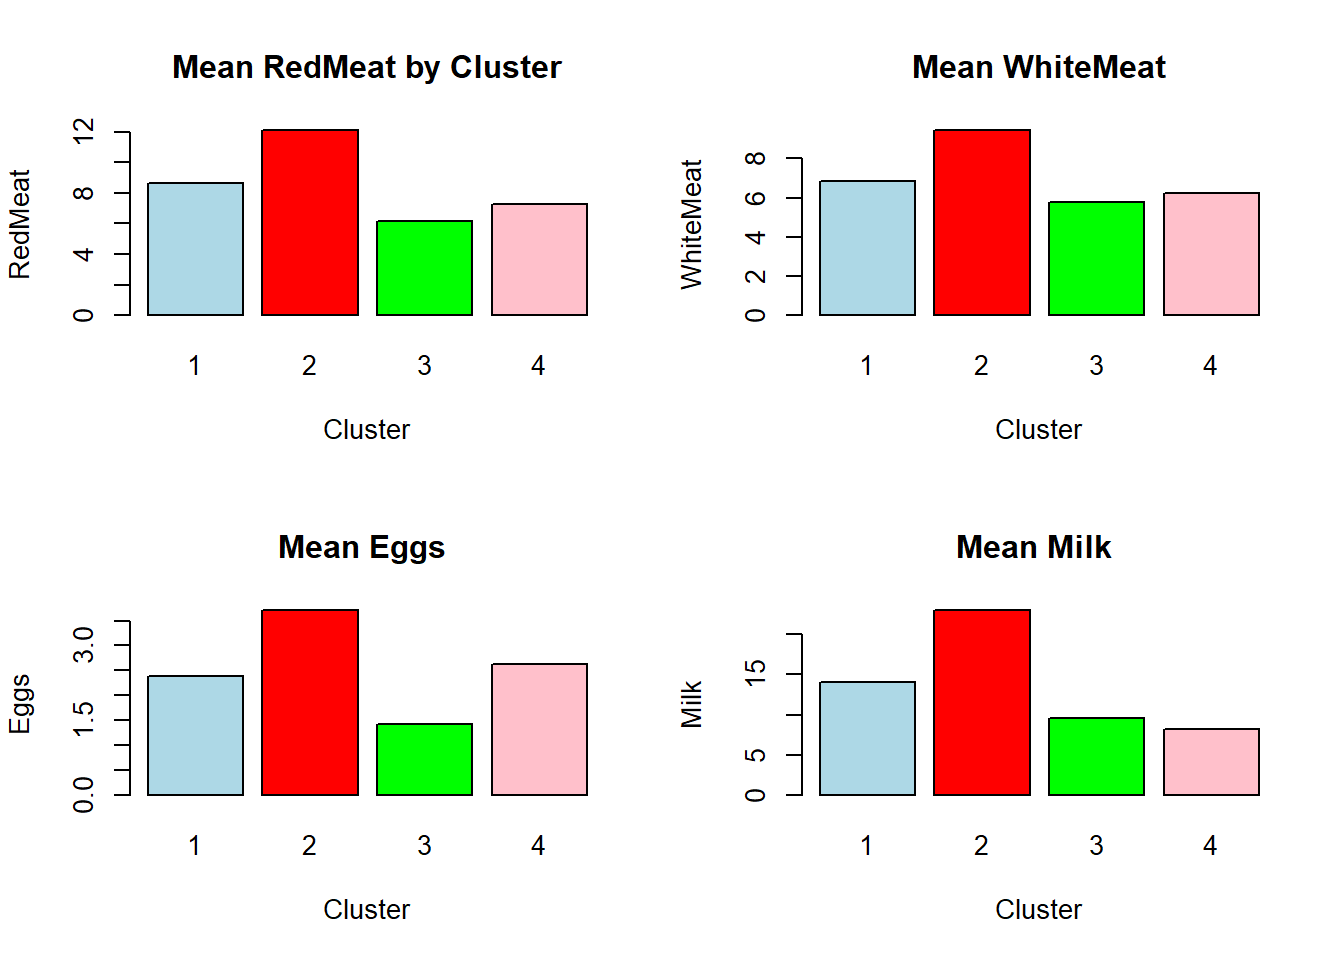
\includegraphics{proyecto.reglasAsociacion_files/figure-beamer/unnamed-chunk-16-1.pdf}

Observamos que se produjeron dos paradas en la ventas, que se
reiniciaron en \emph{2001-01} y \emph{2002-01}

\end{frame}

\begin{frame}[fragile]{Visualiza con distintos gr?ficos el
\emph{dataset}: valores distintos de cada columna (II)}
\protect\hypertarget{visualiza-con-distintos-grficos-el-dataset-valores-distintos-de-cada-columna-ii}{}

\begin{Shaded}
\begin{Highlighting}[]
\NormalTok{plot2 <-}\StringTok{ }\KeywordTok{ggplot}\NormalTok{(online, }\KeywordTok{aes}\NormalTok{(ProductoComprado)) }\OperatorTok{+}\StringTok{ }
\StringTok{  }\KeywordTok{geom_bar}\NormalTok{() }\OperatorTok{+}\StringTok{ }
\StringTok{  }\KeywordTok{xlab}\NormalTok{(}\StringTok{"Item"}\NormalTok{) }\OperatorTok{+}\StringTok{ }\KeywordTok{ylab}\NormalTok{(}\StringTok{"Frecuencia"}\NormalTok{) }\OperatorTok{+}\StringTok{ }
\StringTok{  }\KeywordTok{coord_flip}\NormalTok{(); plot2}
\end{Highlighting}
\end{Shaded}

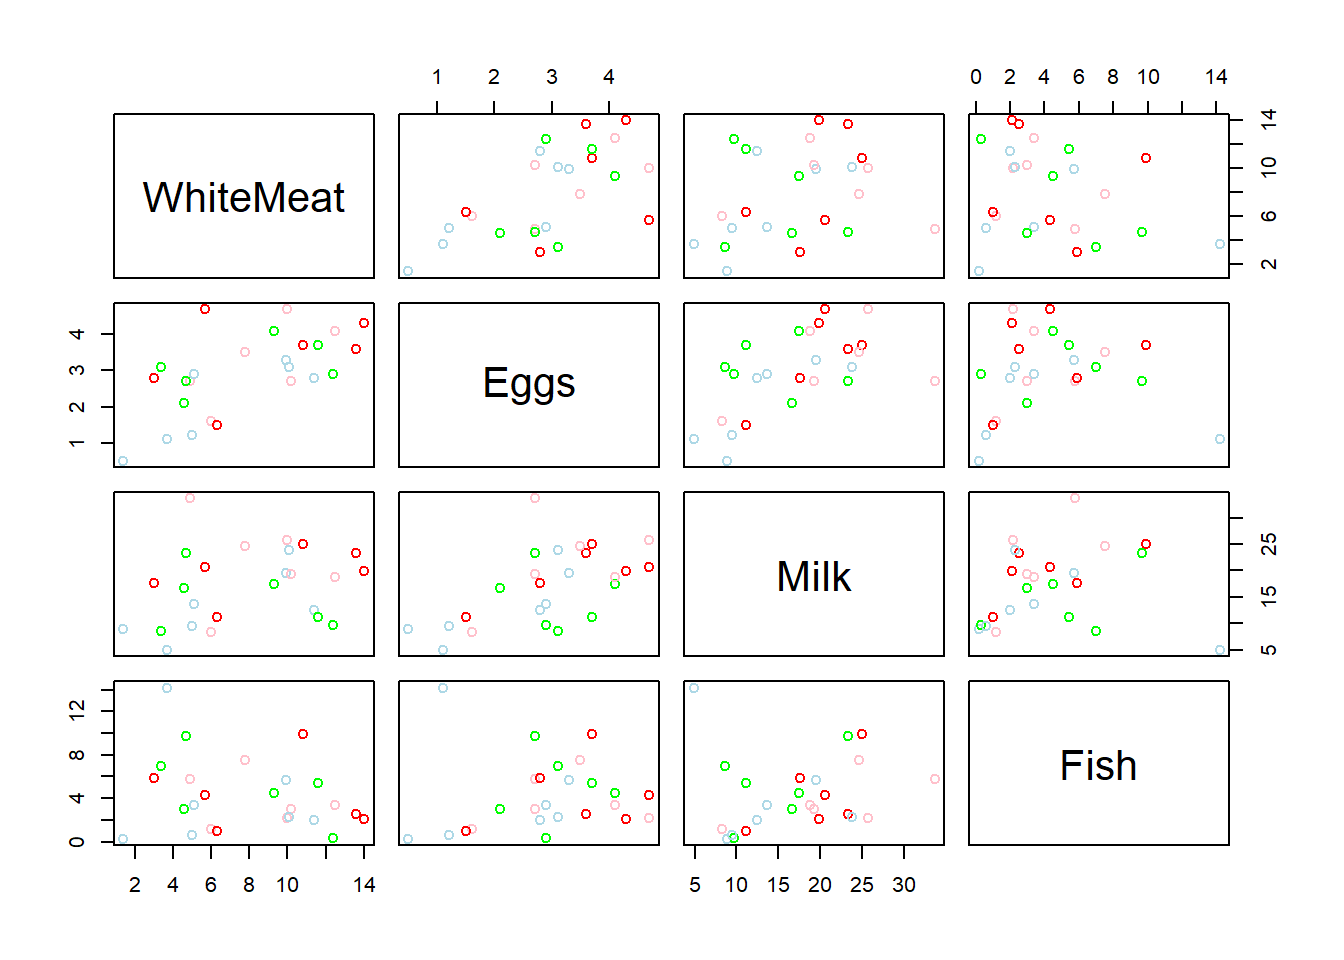
\includegraphics{proyecto.reglasAsociacion_files/figure-beamer/unnamed-chunk-17-1.pdf}

\end{frame}

\begin{frame}[fragile]{Visualiza con distintos gr?ficos el
\emph{dataset}: enfrenta unas variables contra otras para buscar
patrones (I)}
\protect\hypertarget{visualiza-con-distintos-grficos-el-dataset-enfrenta-unas-variables-contra-otras-para-buscar-patrones-i}{}

Puede ser interesante conocer las ventas seg?n el mes o el a?o. Para
ello, debemos manipular el \emph{dataset} original.

A?adimos nuevas columnas, \textbf{\emph{Mes}} y \textbf{\emph{Year}}:

\begin{Shaded}
\begin{Highlighting}[]
\NormalTok{online2 <-}\StringTok{ }\NormalTok{online }\OperatorTok
\StringTok{  }\KeywordTok{mutate}\NormalTok{(}\DataTypeTok{Mes =} \KeywordTok{months}\NormalTok{(Fecha)) }\OperatorTok
\StringTok{  }\KeywordTok{mutate}\NormalTok{(}\DataTypeTok{Year =} \KeywordTok{as.numeric}\NormalTok{(}\KeywordTok{format}\NormalTok{(Fecha,}\StringTok{'%Y'}\NormalTok{)))}
\end{Highlighting}
\end{Shaded}

Ahora podemos agrupar por a?o y visualizar:

\begin{Shaded}
\begin{Highlighting}[]
\NormalTok{plot3 <-}\StringTok{ }\KeywordTok{ggplot}\NormalTok{(online2, }\KeywordTok{aes}\NormalTok{(Year, }\DataTypeTok{fill =} \KeywordTok{as.factor}\NormalTok{(Year))) }\OperatorTok{+}\StringTok{ }
\StringTok{  }\KeywordTok{geom_bar}\NormalTok{() }\OperatorTok{+}\StringTok{ }
\StringTok{  }\KeywordTok{ylab}\NormalTok{(}\StringTok{"Compras"}\NormalTok{) }\OperatorTok{+}\StringTok{ }
\StringTok{  }\KeywordTok{guides}\NormalTok{(}\DataTypeTok{fill=}\KeywordTok{guide_legend}\NormalTok{(}\DataTypeTok{title=}\OtherTok{NULL}\NormalTok{))}

\NormalTok{plot3}
\end{Highlighting}
\end{Shaded}

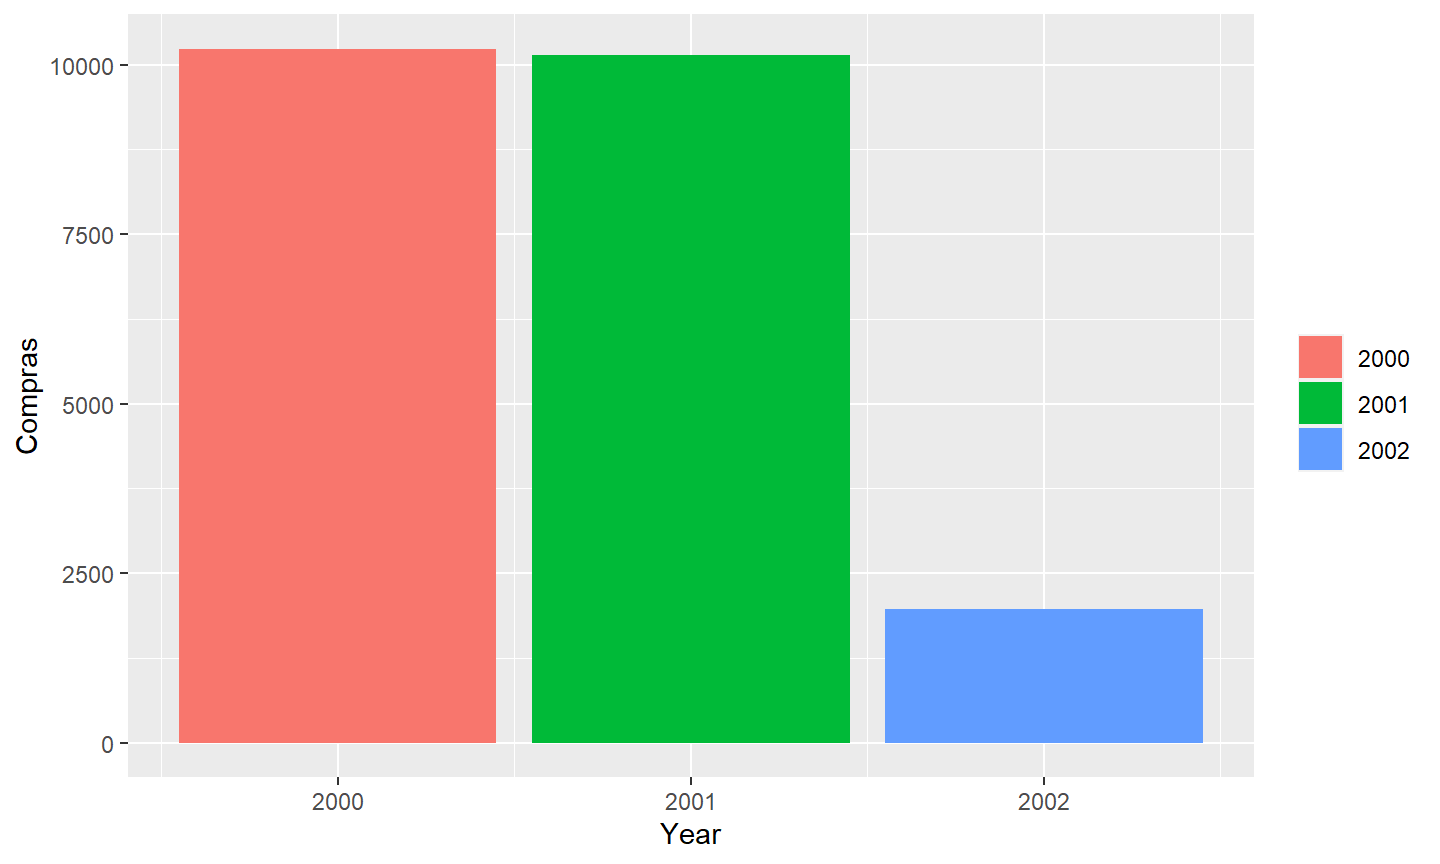
\includegraphics{proyecto.reglasAsociacion_files/figure-beamer/unnamed-chunk-19-1.pdf}

\end{frame}

\begin{frame}[fragile]{Visualiza con distintos gr?ficos el
\emph{dataset}: enfrenta unas variables contra otras para buscar
patrones (II)}
\protect\hypertarget{visualiza-con-distintos-grficos-el-dataset-enfrenta-unas-variables-contra-otras-para-buscar-patrones-ii}{}

Tambi?n ser?a ?til visualizar el n?mero de compras en cada mes por a?o.

\begin{Shaded}
\begin{Highlighting}[]
\NormalTok{plot4 <-}\StringTok{ }\KeywordTok{ggplot}\NormalTok{(online2, }\KeywordTok{aes}\NormalTok{(Mes)) }\OperatorTok{+}\StringTok{ }
\StringTok{  }\KeywordTok{geom_bar}\NormalTok{() }\OperatorTok{+}\StringTok{ }
\StringTok{  }\KeywordTok{facet_wrap}\NormalTok{(}\OperatorTok{~}\StringTok{ }\NormalTok{Year) }\OperatorTok{+}\StringTok{ }
\StringTok{  }\KeywordTok{theme}\NormalTok{(}\DataTypeTok{axis.text.x =} \KeywordTok{element_text}\NormalTok{(}\DataTypeTok{angle =} \DecValTok{45}\NormalTok{)) }\OperatorTok{+}
\StringTok{  }\KeywordTok{labs}\NormalTok{(}\DataTypeTok{title =} \StringTok{"Compras por mes en cada a?o"}\NormalTok{, }\DataTypeTok{x =} \OtherTok{NULL}\NormalTok{, }\DataTypeTok{y =} \StringTok{"Compras"}\NormalTok{)}

\NormalTok{plot4}
\end{Highlighting}
\end{Shaded}

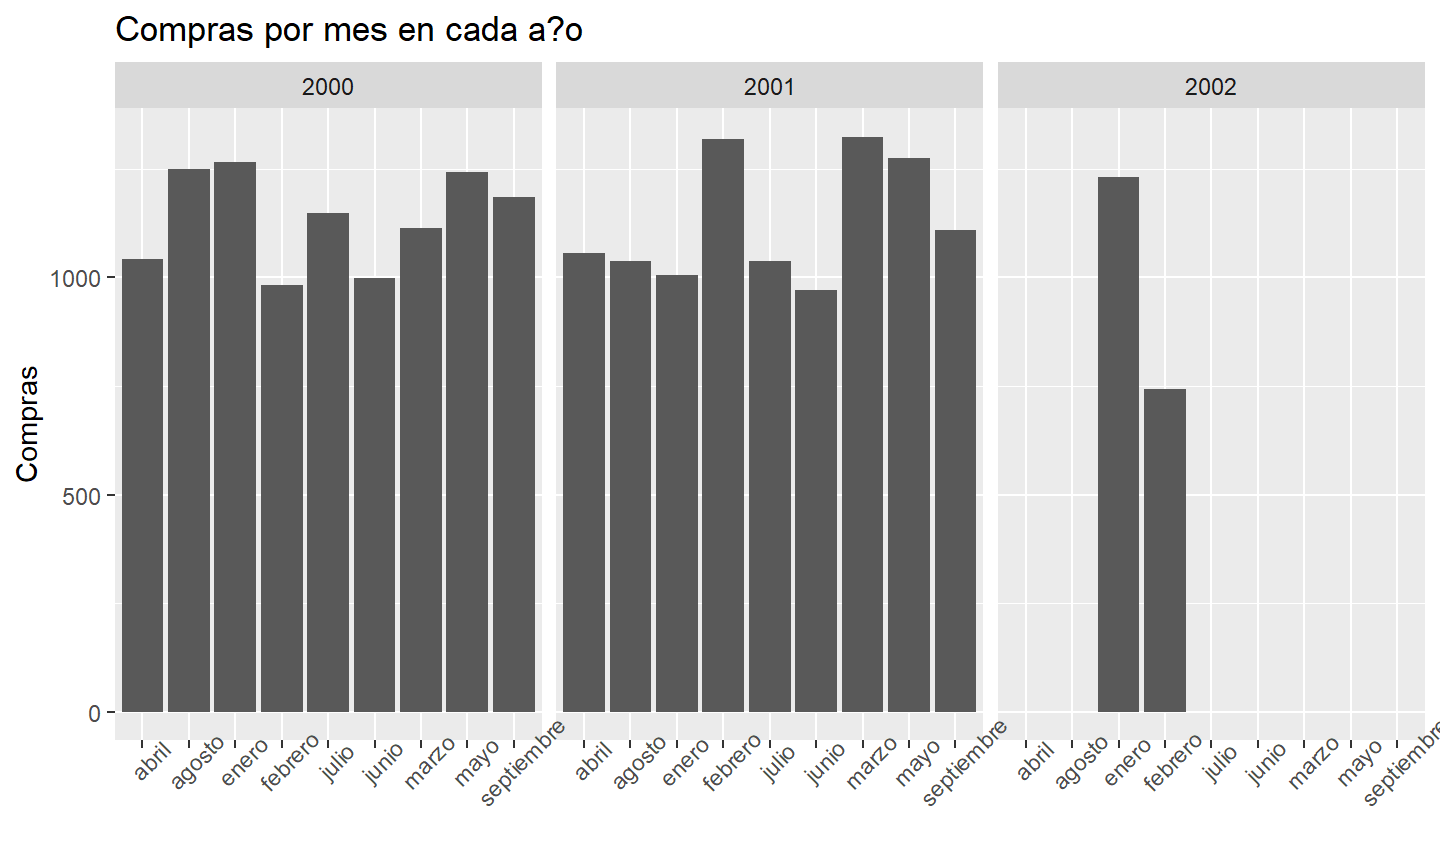
\includegraphics{proyecto.reglasAsociacion_files/figure-beamer/unnamed-chunk-20-1.pdf}

\end{frame}

\begin{frame}[fragile]{Usa \texttt{split} para construir a partir del
\emph{dataset} una lista con nombre
\textbf{\emph{lista.compra.usuarios}} en la que cada elemento de la
lista es cada comprador junto con todos los productos que ha comprado}
\protect\hypertarget{usa-split-para-construir-a-partir-del-dataset-una-lista-con-nombre-lista.compra.usuarios-en-la-que-cada-elemento-de-la-lista-es-cada-comprador-junto-con-todos-los-productos-que-ha-comprado}{}

Tras dividir por comprador, uso \texttt{lapply()} para quedarme con los
productos.

\begin{Shaded}
\begin{Highlighting}[]
\NormalTok{lista.compra.usuarios <-}\StringTok{ }\KeywordTok{split}\NormalTok{(online, online}\OperatorTok{$}\NormalTok{IDcomprador)}
\NormalTok{lista.compra.usuarios <-}\StringTok{ }\KeywordTok{lapply}\NormalTok{(lista.compra.usuarios, }
                                \ControlFlowTok{function}\NormalTok{(x) x}\OperatorTok{$}\NormalTok{ProductoComprado)}
\NormalTok{lista.compra.usuarios[}\DecValTok{1}\NormalTok{]}
\end{Highlighting}
\end{Shaded}

\begin{verbatim}
## $`1`
##  [1] "yogurt"            "pork"              "sandwich bags"    
##  [4] "lunch meat"        "all- purpose"      "flour"            
##  [7] "soda"              "butter"            "vegetables"       
## [10] "beef"              "aluminum foil"     "all- purpose"     
## [13] "dinner rolls"      "shampoo"           "all- purpose"     
## [16] "mixes"             "soap"              "laundry detergent"
## [19] "ice cream"         "dinner rolls"
\end{verbatim}

\end{frame}

\begin{frame}[fragile]{Hacer \texttt{summary} y contar usuarios de
\textbf{\emph{lista.compra.usuarios}}}
\protect\hypertarget{hacer-summary-y-contar-usuarios-de-lista.compra.usuarios}{}

\begin{Shaded}
\begin{Highlighting}[]
\KeywordTok{head}\NormalTok{(}\KeywordTok{summary}\NormalTok{(lista.compra.usuarios))}
\end{Highlighting}
\end{Shaded}

\begin{verbatim}
##   Length Class  Mode     
## 1 20     -none- character
## 2 23     -none- character
## 3 31     -none- character
## 4  6     -none- character
## 5 27     -none- character
## 6 28     -none- character
\end{verbatim}

\begin{Shaded}
\begin{Highlighting}[]
\KeywordTok{length}\NormalTok{(lista.compra.usuarios)}
\end{Highlighting}
\end{Shaded}

\begin{verbatim}
## [1] 1139
\end{verbatim}

\end{frame}

\begin{frame}[fragile]{Eliminar duplicados, contar cu?ntos usuarios hay
en la lista despu?s de eliminar duplicados en la
\textbf{\emph{lista.compra.usuarios}} y convertir a tipo de datos
transacciones}
\protect\hypertarget{eliminar-duplicados-contar-cuntos-usuarios-hay-en-la-lista-despus-de-eliminar-duplicados-en-la-lista.compra.usuarios-y-convertir-a-tipo-de-datos-transacciones}{}

\begin{itemize}
\tightlist
\item
  Podemos usar \texttt{unique()} para quitar los duplicados, aunque no
  hay:
\end{itemize}

\begin{Shaded}
\begin{Highlighting}[]
\KeywordTok{length}\NormalTok{(lista.compra.usuarios) }\OperatorTok{==}\StringTok{ }\KeywordTok{length}\NormalTok{(}\KeywordTok{unique}\NormalTok{(lista.compra.usuarios))}
\end{Highlighting}
\end{Shaded}

\begin{verbatim}
## [1] TRUE
\end{verbatim}

\begin{itemize}
\tightlist
\item
  Convertimos a tipo \emph{transacciones}:
\end{itemize}

\begin{Shaded}
\begin{Highlighting}[]
\NormalTok{Tlista.compra.usuarios <-}\StringTok{ }\KeywordTok{as}\NormalTok{(lista.compra.usuarios, }\StringTok{"transactions"}\NormalTok{)}
\end{Highlighting}
\end{Shaded}

\end{frame}

\begin{frame}[fragile]{Hacer \texttt{inspect} de los dos primeros
valores}
\protect\hypertarget{hacer-inspect-de-los-dos-primeros-valores}{}

\begin{Shaded}
\begin{Highlighting}[]
\KeywordTok{inspect}\NormalTok{(Tlista.compra.usuarios[}\DecValTok{1}\OperatorTok{:}\DecValTok{2}\NormalTok{])}
\end{Highlighting}
\end{Shaded}

\begin{verbatim}
##     items                          transactionID
## [1] {all- purpose,                              
##      aluminum foil,                             
##      beef,                                      
##      butter,                                    
##      dinner rolls,                              
##      flour,                                     
##      ice cream,                                 
##      laundry detergent,                         
##      lunch meat,                                
##      mixes,                                     
##      pork,                                      
##      sandwich bags,                             
##      shampoo,                                   
##      soap,                                      
##      soda,                                      
##      vegetables,                                
##      yogurt}                                   1
## [2] {aluminum foil,                             
##      cereals,                                   
##      cheeses,                                   
##      dishwashing liquid/detergent,              
##      hand soap,                                 
##      individual meals,                          
##      laundry detergent,                         
##      milk,                                      
##      mixes,                                     
##      sandwich bags,                             
##      shampoo,                                   
##      toilet paper,                              
##      tortillas,                                 
##      vegetables,                                
##      waffles,                                   
##      yogurt}                                   2
\end{verbatim}

\end{frame}

\begin{frame}[fragile]{Buscar ayuda de \texttt{itemFrequencyPlot} para
visualizar las \(20\) transacciones m?s frecuentes}
\protect\hypertarget{buscar-ayuda-de-itemfrequencyplot-para-visualizar-las-20-transacciones-ms-frecuentes}{}

La clave est? en el par?metro \textbf{\emph{topN}}:

\begin{Shaded}
\begin{Highlighting}[]
\KeywordTok{itemFrequencyPlot}\NormalTok{(Tlista.compra.usuarios, }\DataTypeTok{topN =} \DecValTok{20}\NormalTok{)}
\end{Highlighting}
\end{Shaded}

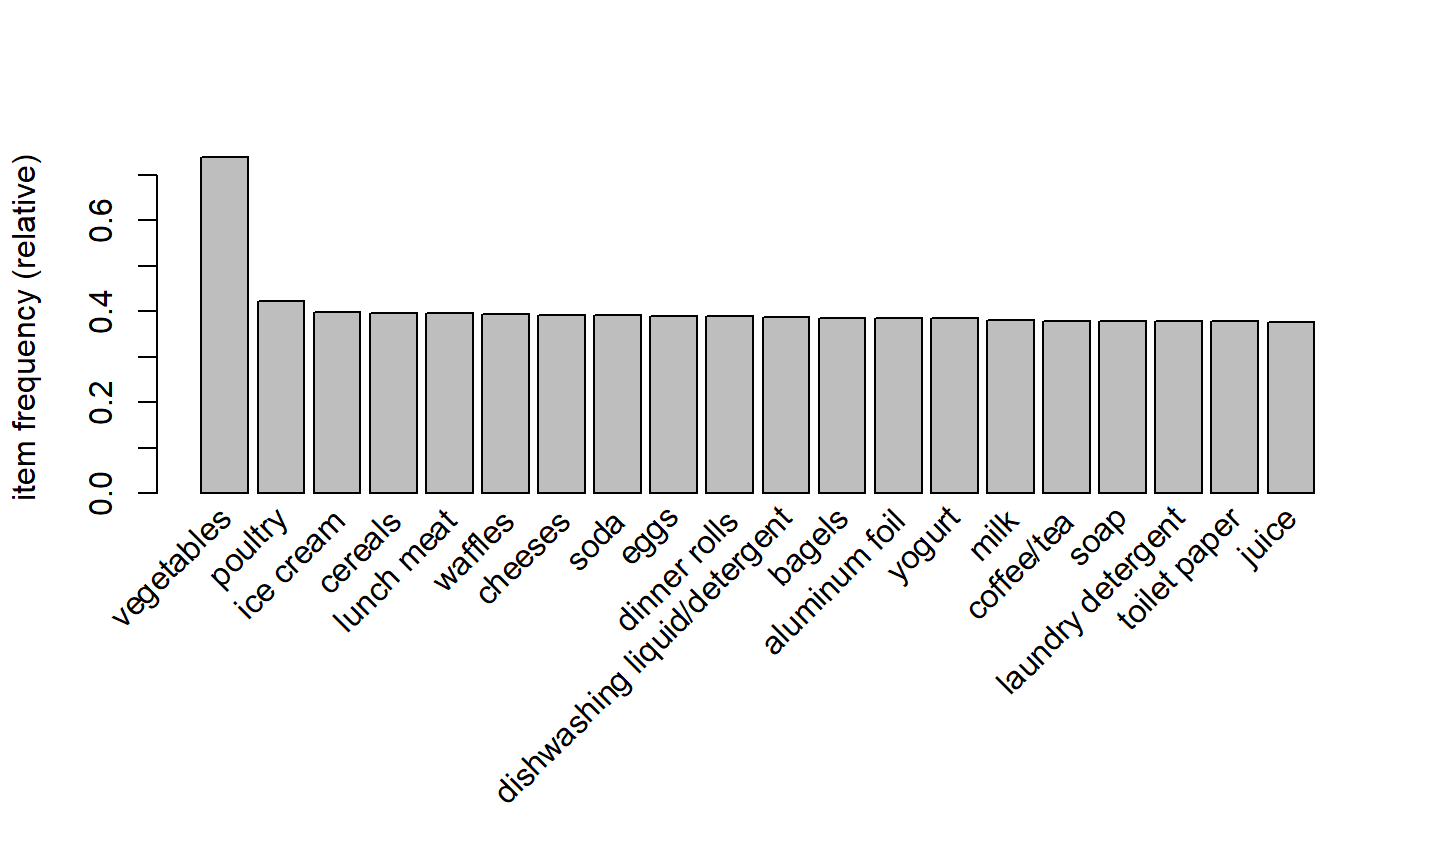
\includegraphics{proyecto.reglasAsociacion_files/figure-beamer/unnamed-chunk-26-1.pdf}

\end{frame}

\begin{frame}[fragile]{Generar las reglas de asociaci?n con \(80\)\% de
confianza y \(15\)\% de soporte}
\protect\hypertarget{generar-las-reglas-de-asociacin-con-80-de-confianza-y-15-de-soporte}{}

Usamos la funci?n \texttt{apriori()} para generar las reglas:

\begin{Shaded}
\begin{Highlighting}[]
\NormalTok{reglas <-}\StringTok{ }\KeywordTok{apriori}\NormalTok{(Tlista.compra.usuarios, }
                  \DataTypeTok{parameter =} \KeywordTok{list}\NormalTok{(}\DataTypeTok{supp =} \FloatTok{0.15}\NormalTok{, }\DataTypeTok{conf =} \FloatTok{0.8}\NormalTok{))}
\end{Highlighting}
\end{Shaded}

\begin{verbatim}
## Apriori
## 
## Parameter specification:
##  confidence minval smax arem  aval originalSupport maxtime support minlen
##         0.8    0.1    1 none FALSE            TRUE       5    0.15      1
##  maxlen target  ext
##      10  rules TRUE
## 
## Algorithmic control:
##  filter tree heap memopt load sort verbose
##     0.1 TRUE TRUE  FALSE TRUE    2    TRUE
## 
## Absolute minimum support count: 170 
## 
## set item appearances ...[0 item(s)] done [0.00s].
## set transactions ...[38 item(s), 1139 transaction(s)] done [0.00s].
## sorting and recoding items ... [38 item(s)] done [0.00s].
## creating transaction tree ... done [0.00s].
## checking subsets of size 1 2 3 done [0.00s].
## writing ... [22 rule(s)] done [0.00s].
## creating S4 object  ... done [0.00s].
\end{verbatim}

\end{frame}

\begin{frame}[fragile]{Ver las reglas generadas y ordenalas por
\textbf{\emph{lift}}. Guarda el resultado en una variable nueva (I)}
\protect\hypertarget{ver-las-reglas-generadas-y-ordenalas-por-lift.-guarda-el-resultado-en-una-variable-nueva-i}{}

\begin{Shaded}
\begin{Highlighting}[]
\NormalTok{reglas.por.lift <-}\StringTok{ }\KeywordTok{sort}\NormalTok{(reglas, }\DataTypeTok{by =} \StringTok{"lift"}\NormalTok{) }
\end{Highlighting}
\end{Shaded}

\begin{Shaded}
\begin{Highlighting}[]
\KeywordTok{inspect}\NormalTok{(reglas.por.lift)}
\end{Highlighting}
\end{Shaded}

\begin{verbatim}
##      lhs                                       rhs          support  
## [1]  {eggs,yogurt}                          => {vegetables} 0.1571554
## [2]  {dinner rolls,eggs}                    => {vegetables} 0.1562774
## [3]  {dishwashing liquid/detergent,eggs}    => {vegetables} 0.1536435
## [4]  {cereals,laundry detergent}            => {vegetables} 0.1510097
## [5]  {cheeses,eggs}                         => {vegetables} 0.1501317
## [6]  {eggs,poultry}                         => {vegetables} 0.1553995
## [7]  {cereals,eggs}                         => {vegetables} 0.1510097
## [8]  {aluminum foil,yogurt}                 => {vegetables} 0.1527656
## [9]  {mixes,poultry}                        => {vegetables} 0.1562774
## [10] {dishwashing liquid/detergent,poultry} => {vegetables} 0.1597893
## [11] {lunch meat,waffles}                   => {vegetables} 0.1571554
## [12] {lunch meat,poultry}                   => {vegetables} 0.1580334
## [13] {poultry,sugar}                        => {vegetables} 0.1518876
## [14] {eggs,soda}                            => {vegetables} 0.1580334
## [15] {poultry,yogurt}                       => {vegetables} 0.1527656
## [16] {eggs}                                 => {vegetables} 0.3266023
## [17] {yogurt}                               => {vegetables} 0.3195786
## [18] {dinner rolls,poultry}                 => {vegetables} 0.1615452
## [19] {sugar}                                => {vegetables} 0.2976295
## [20] {laundry detergent}                    => {vegetables} 0.3090430
## [21] {sandwich loaves}                      => {vegetables} 0.2827041
## [22] {aluminum foil}                        => {vegetables} 0.3107989
##      confidence coverage  lift     count
## [1]  0.8994975  0.1747147 1.216779 179  
## [2]  0.8989899  0.1738367 1.216092 178  
## [3]  0.8974359  0.1712028 1.213990 175  
## [4]  0.8911917  0.1694469 1.205543 172  
## [5]  0.8860104  0.1694469 1.198534 171  
## [6]  0.8805970  0.1764706 1.191211 177  
## [7]  0.8643216  0.1747147 1.169195 172  
## [8]  0.8613861  0.1773486 1.165224 174  
## [9]  0.8599034  0.1817384 1.163218 178  
## [10] 0.8544601  0.1870061 1.155855 182  
## [11] 0.8523810  0.1843723 1.153043 179  
## [12] 0.8490566  0.1861282 1.148546 180  
## [13] 0.8480392  0.1791045 1.147169 173  
## [14] 0.8450704  0.1870061 1.143153 180  
## [15] 0.8446602  0.1808604 1.142599 174  
## [16] 0.8378378  0.3898156 1.133370 372  
## [17] 0.8310502  0.3845478 1.124188 364  
## [18] 0.8288288  0.1949078 1.121183 184  
## [19] 0.8248175  0.3608428 1.115757 339  
## [20] 0.8167053  0.3784021 1.104783 352  
## [21] 0.8090452  0.3494293 1.094421 322  
## [22] 0.8082192  0.3845478 1.093304 354
\end{verbatim}

\end{frame}

\begin{frame}[fragile]{Elimina todas las reglas redundantes. Calcula el
\% de reglas redundantes que hab?a}
\protect\hypertarget{elimina-todas-las-reglas-redundantes.-calcula-el-de-reglas-redundantes-que-haba}{}

\begin{itemize}
\tightlist
\item
  Eliminamos las reglas redundantes:
\end{itemize}

\begin{Shaded}
\begin{Highlighting}[]
\NormalTok{reglas.no.redun.lift <-}\StringTok{ }\NormalTok{reglas.por.lift[}\OperatorTok{!}\KeywordTok{is.redundant}\NormalTok{(reglas.por.lift)]}
\end{Highlighting}
\end{Shaded}

\begin{itemize}
\tightlist
\item
  Aunque no hay reglas redundantes, el \% de reglas redundantes podr?a
  calcularse as?:
\end{itemize}

\(porcentaje = \frac{reglas.redundantes}{total.reglas} * 100\)

donde

\(reglas.redundantes =\) \texttt{length(reglas.por.lift)} -
\texttt{lenght(reglas.no.redun.lift)}

y \(total.reglas =\) \texttt{length(reglas.por.lift)}

\end{frame}

\begin{frame}[fragile]{Dibuja las reglas ordenadas y no redundantes
usando paquete \textbf{\emph{arulesViz}} (I)}
\protect\hypertarget{dibuja-las-reglas-ordenadas-y-no-redundantes-usando-paquete-arulesviz-i}{}

\begin{Shaded}
\begin{Highlighting}[]
\KeywordTok{library}\NormalTok{(arulesViz)}
\KeywordTok{plot}\NormalTok{(reglas.no.redun.lift, }\DataTypeTok{method =} \StringTok{"graph"}\NormalTok{)}
\end{Highlighting}
\end{Shaded}

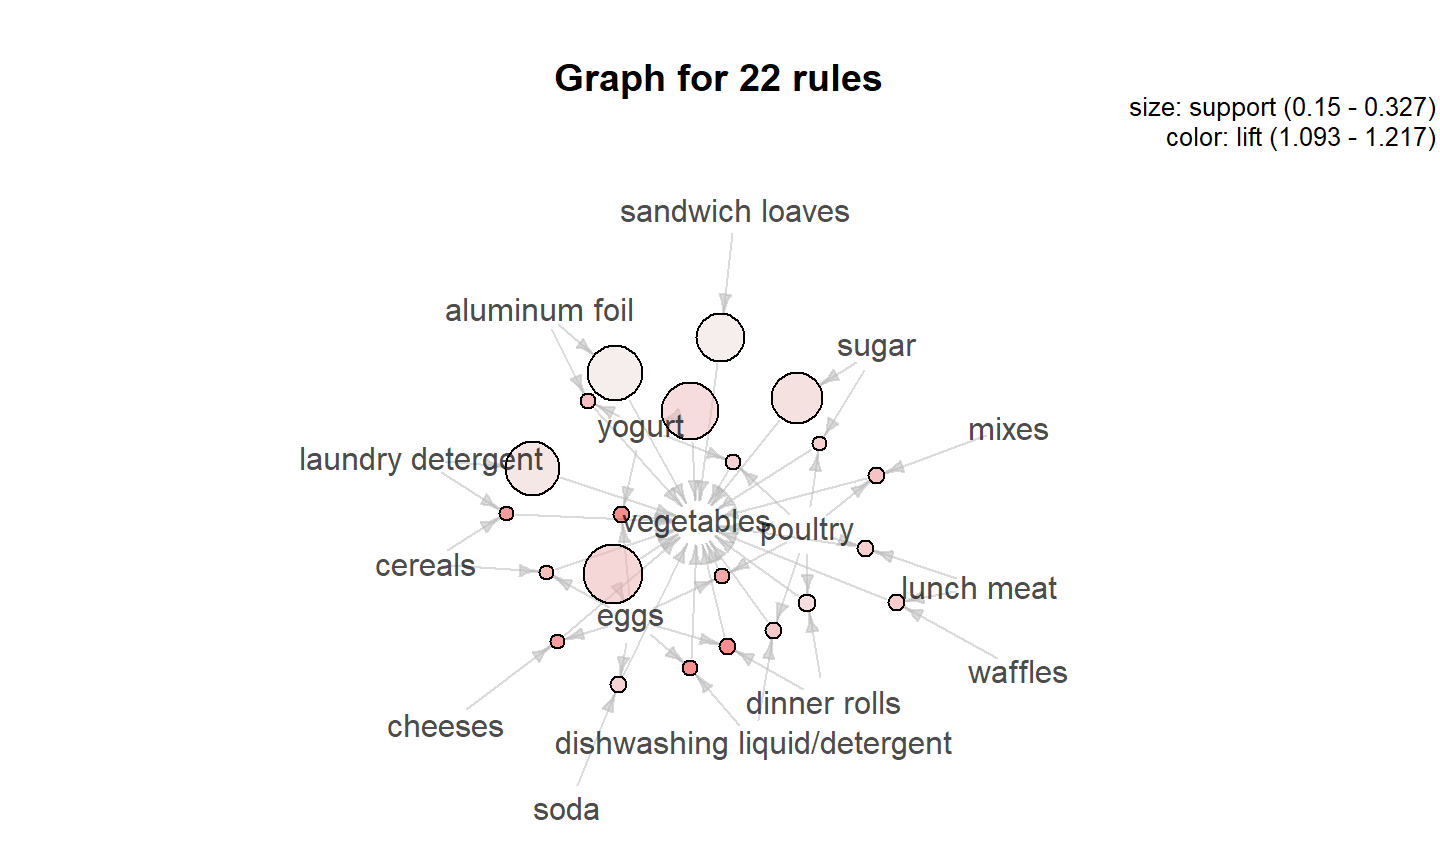
\includegraphics{proyecto.reglasAsociacion_files/figure-beamer/unnamed-chunk-31-1.pdf}

\end{frame}

\begin{frame}[fragile]{Dibuja las reglas ordenadas y no redundantes
usando paquete \textbf{\emph{arulesViz}} (II)}
\protect\hypertarget{dibuja-las-reglas-ordenadas-y-no-redundantes-usando-paquete-arulesviz-ii}{}

\begin{Shaded}
\begin{Highlighting}[]
\KeywordTok{plot}\NormalTok{(reglas.no.redun.lift)}
\end{Highlighting}
\end{Shaded}

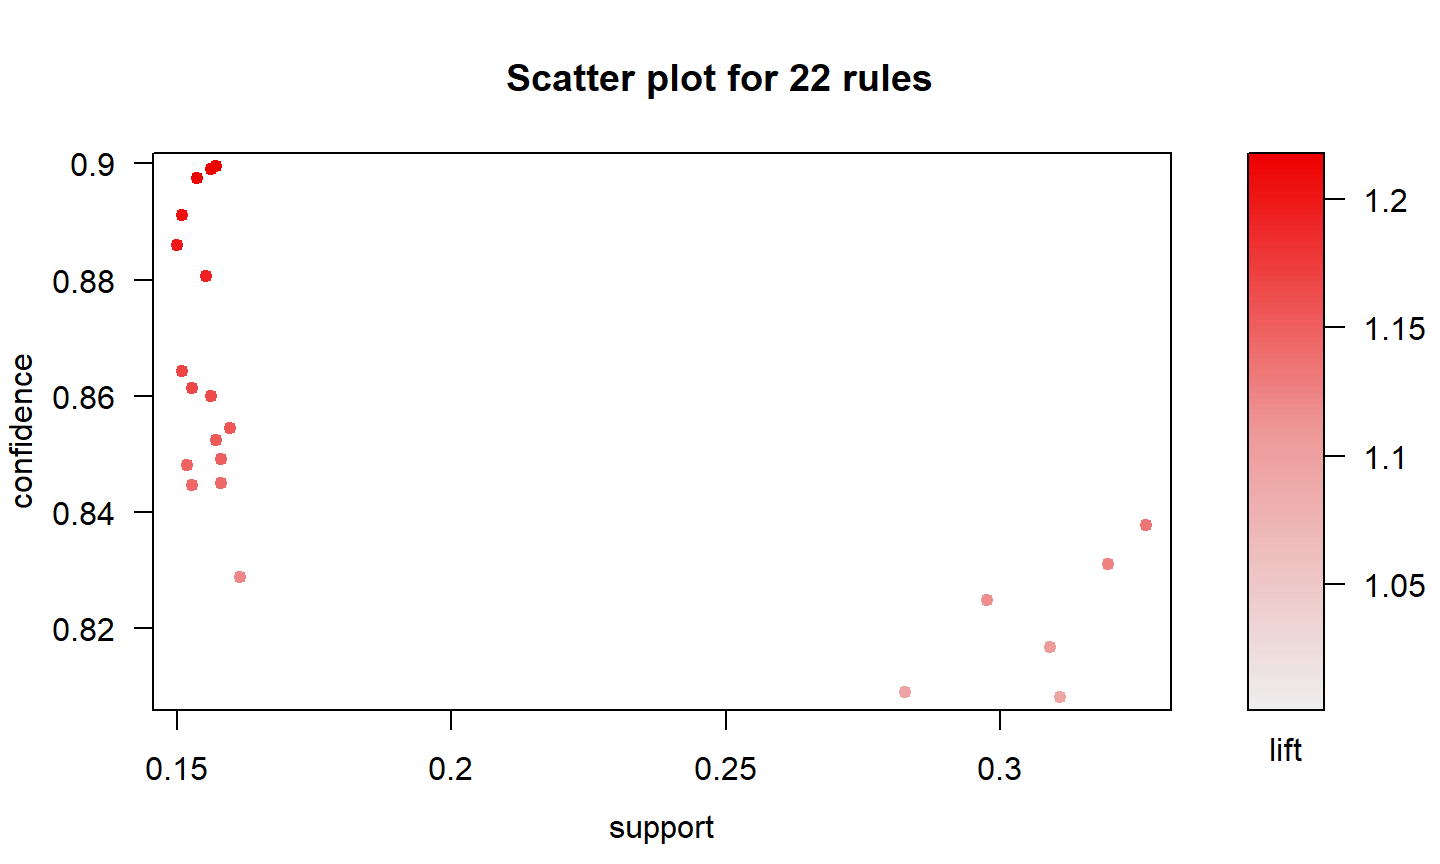
\includegraphics{proyecto.reglasAsociacion_files/figure-beamer/unnamed-chunk-32-1.pdf}

\end{frame}

\begin{frame}[fragile]{Aplicar la noci?n de \emph{afinidad} introducida
en clase}
\protect\hypertarget{aplicar-la-nocin-de-afinidad-introducida-en-clase}{}

Usamos la funci?n \texttt{affinity()} para calcular una matriz de
afinidad entre los \emph{items}. S?lo se muestra una submatriz de
\(9\times5\)

\begin{Shaded}
\begin{Highlighting}[]
\KeywordTok{affinity}\NormalTok{(Tlista.compra.usuarios)[}\DecValTok{1}\OperatorTok{:}\DecValTok{9}\NormalTok{, }\DecValTok{1}\OperatorTok{:}\DecValTok{5}\NormalTok{]}
\end{Highlighting}
\end{Shaded}

\begin{verbatim}
##               all- purpose aluminum foil    bagels      beef    butter
## all- purpose     0.0000000     0.2609329 0.2460432 0.2394775 0.2477876
## aluminum foil    0.2609329     0.0000000 0.2802920 0.2664714 0.2438316
## bagels           0.2460432     0.2802920 0.0000000 0.2587209 0.2525547
## beef             0.2394775     0.2664714 0.2587209 0.0000000 0.2085714
## butter           0.2477876     0.2438316 0.2525547 0.2085714 0.0000000
## cereals          0.2436261     0.2700000 0.2624113 0.2798834 0.2446352
## cheeses          0.2403983     0.2797101 0.2756133 0.2637681 0.2668622
## coffee/tea       0.2413295     0.2626996 0.2478510 0.2306590 0.2369186
## dinner rolls     0.2554113     0.2731214 0.2510638 0.2536023 0.2510885
\end{verbatim}

\end{frame}

\begin{frame}{Investigar alg?n otro paquete \emph{R} relacionado con
reglas de asociaci?n.~Explicar su uso con un \emph{dataset} y ejemplos
(I)}
\protect\hypertarget{investigar-algn-otro-paquete-r-relacionado-con-reglas-de-asociacin.-explicar-su-uso-con-un-dataset-y-ejemplos-i}{}

El paquete \textbf{\emph{RWeka}} es una interfaz de \emph{R} para
\emph{Weka}.

\emph{Weka} es una colecci?n de algoritmos de \emph{machine learning}
para tareas \emph{data mining}.

Est? escrito en \emph{Java} y tiene herramientas para preprocesar datos,
clasficaci?n, regresi?n, \emph{clustering}, \textbf{reglas de
asociaci?n} y visualizaci?n.

Se puede encontrar m?s informaci?n en:\\
\url{https://cran.r-project.org/web/packages/RWeka/RWeka.pdf}~\\
\url{https://rdrr.io/cran/RWeka/man/Weka_associators.html}

\end{frame}

\begin{frame}[fragile]{Investigar alg?n otro paquete \emph{R}
relacionado con reglas de asociaci?n.~Explicar su uso con un
\emph{dataset} y ejemplos (II)}
\protect\hypertarget{investigar-algn-otro-paquete-r-relacionado-con-reglas-de-asociacin.-explicar-su-uso-con-un-dataset-y-ejemplos-ii}{}

\begin{itemize}
\tightlist
\item
  Cargamos el \emph{dataset} mediante la funcion \texttt{read.arff()}:
\end{itemize}

\end{frame}

\end{document}
